\setchapterpreamble[u]{\margintoc}
\chapter{Self-Driving with Statistics}
\labch{driving}

\textit{"We think of automation as a machine doing a task that a human used to do... you might think that means a human does nothing. But in fact there's abundant literature that shows the human is not incurring no workload, the human is now doing a different task and that task tends to be monitoring, a vigilance task, looking for rare events...that is a task that humans are not well-equipped to do." - Dr. Michael Nees, 2021} \cite{nees2021}


\section{The Dangers of Semi-Autonomy}

Two hundred years ago, horses were the most sophisticated mode of transportation. They possessed an innate ability to navigate terrain and avoid obstacles, even without a human rider at the reins. People often took comfort in the horse's natural instincts, which allowed for moments of respite during long journeys. Fast forward to today, where we have vehicles that claim to possess similar levels of autonomy, but with significantly more horsepower (pun intended).

One might be tempted to compare these self-driving cars to our trusty equine friends, imagining a world where vehicles, like horses, can be left to their own devices. Alas, this comparison is a misleading one, as it creates the illusion that our self-driving cars are more capable than they currently are.

The National Highway Traffic Safety Administration (NHTSA) has devised a six-level classification system to describe vehicle autonomy, ranging from Level 0 (no automation) to Level 5 (full automation). Most commercially available vehicles today hover between Levels 2 and 3, providing advanced driver assistance but requiring constant human oversight. This semi-autonomous state can lull drivers into a false sense of security, prompting them to disengage from the driving task in a manner that might have been acceptable during the days of horse-drawn carriages but is decidedly dangerous in the modern era.

\begin{pdf}
\begin{marginfigure}[-5.5cm]
        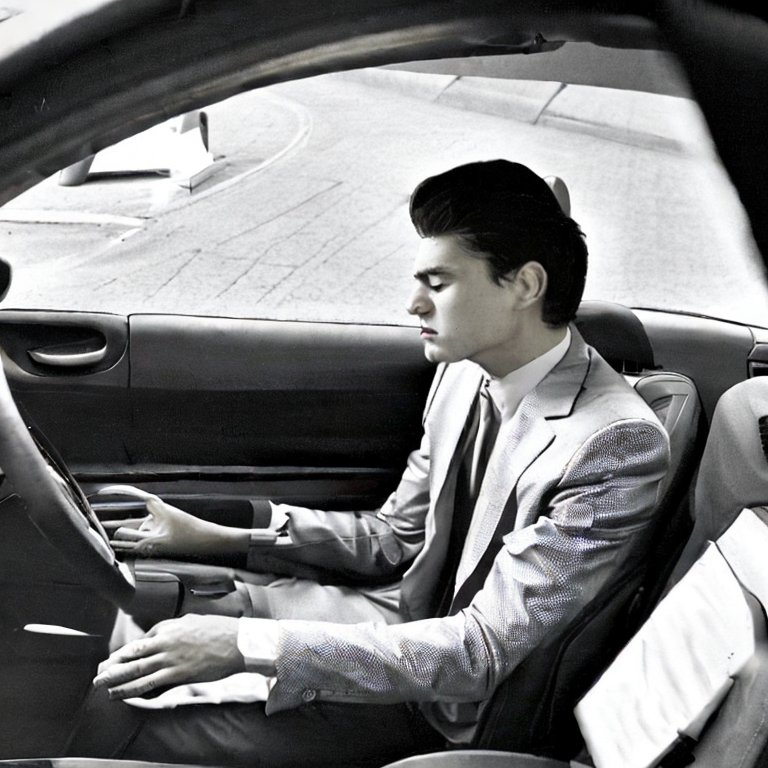
\includegraphics{asleep}
        \caption{"style a person in a business suit asleep at the wheel of a car AP" made with Stable Diffusion 2.1}
        \labfig{asleep}
\end{marginfigure}
\end{pdf}

In his book "Robot Take the Wheel," author Jason Torchinsky offers a compelling argument against semi-autonomy, dubbing it "stupid" in a section bearing the same name. Torchinsky highlights the impracticality of expecting a driver who has relinquished control to a semi-autonomous system to suddenly take over in a moment of crisis. Manufacturer warnings, while intended to encourage drivers to stay attentive, often go unheeded, creating a precarious situation where those behind the wheel are ill-prepared to intervene when the technology falters.\sidecite{torchinskyboeckmann2019}

The world of transportation extends beyond the realm of four-wheeled automobiles. The skies above host a veritable ballet of commercial aircraft, which rely on sophisticated autopilot systems to ferry passengers and cargo across vast distances. These systems differ in important ways from automobile autopilot and have significantly different infrastructure (not to mention terrain, or lack thereof).In aviation, autopilots demand constant monitoring and communication between the pilot, the aircraft, and air traffic control. In many ways, the intricacies and collaboration required for safe air travel can serve as a model for understanding the complexities of developing and implementing truly autonomous ground vehicles.

\section{Comparing Autopilot Systems}

At a glance, the autopilot systems in airplanes and Teslas may seem to share common goals: both strive to provide increased safety, efficiency, and convenience. However, the similarities largely end there, as the underlying technologies and the environments in which they operate diverge significantly.

Commercial airplanes, for example, are equipped with highly sophisticated autopilot systems capable of managing tasks such as altitude, speed, and heading control. In contrast, Tesla's ADAS, while advanced, is focused primarily on lane keeping, adaptive cruise control, and collision avoidance. Furthermore, the aviation industry has a long history of integrating automation with well-established regulations, procedures, and training, whereas the automotive industry is still in the early stages of defining standards and best practices for autonomous vehicles.

One critical aspect of aircraft autopilot systems is the need for seamless communication and coordination with external systems, such as air traffic control (ATC) and other aircraft. This level of coordination ensures that each plane maintains a safe distance from others, follows established routes, and adheres to ATC instructions.

On the other hand, vehicles like Teslas currently have limited means of communication with external systems, relying instead on onboard sensors and mapping data to navigate the environment. As autonomous vehicle technology advances, however, it is anticipated that vehicle-to-vehicle (V2V) and vehicle-to-infrastructure (V2I) communication will become increasingly important for coordinating traffic flow and maintaining safety.

\begin{pdf}
\begin{marginfigure}[-5.5cm]
        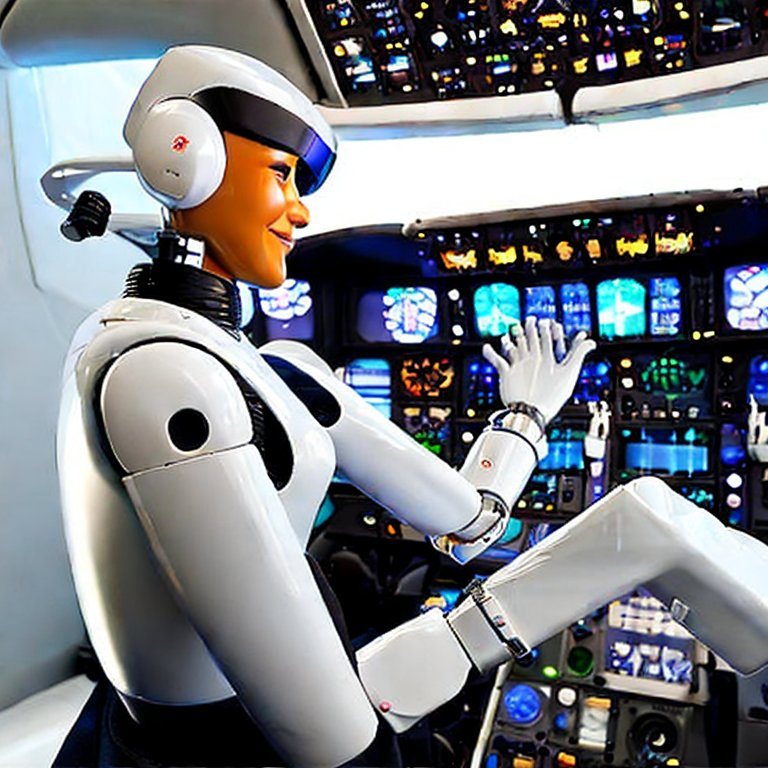
\includegraphics{pilot}
        \caption{"a robot pilot at the helm of a commercial airliner, being served by a human flight attendant" made with Stable Diffusion 2.1}
        \labfig{pilot}
\end{marginfigure}
\end{pdf}

Despite the advanced nature of aircraft autopilot systems, pilots are still required to maintain a constant vigil, monitoring the system and intervening when necessary. This level of human oversight is not only mandated by regulations but also reinforced through rigorous training and the understanding that even the most advanced systems can fail.

In contrast, drivers of vehicles equipped with ADAS, such as Teslas, often face the temptation to over-rely on the technology and disengage from the driving task, as discussed in the previous section. This discrepancy highlights the need for clear guidelines and education on the proper use of semi-autonomous systems in cars, to ensure that drivers remain vigilant and prepared to intervene when needed.

\section{Who Should The Car Kill?}

In this section, we delve into the ethical dilemmas that arise when designing autonomous vehicles. We will discuss the Trolley Problem and its application to autonomous decision-making, as well as the legal and moral considerations of outsourcing responsibility to machines.

The Trolley Problem, a classic thought experiment in ethics, poses a hypothetical scenario where an individual must choose between two undesirable outcomes, often involving the deaths of different groups of people. In the context of autonomous vehicles, the Trolley Problem raises the question of how a self-driving car should prioritize the safety of its occupants, pedestrians, and other road users in situations where an accident is unavoidable.

As developers of autonomous vehicles grapple with these ethical quandaries, they must decide what values and priorities to embed in their algorithms. Should a self-driving car prioritize minimizing overall harm, protecting its passengers, or adhering to specific legal and moral rules? The choices made in designing these systems will have profound implications for society, as they will determine how autonomous vehicles respond in life-or-death situations.

The advent of autonomous vehicles raises complex questions about responsibility and liability. If a self-driving car is involved in an accident, who should be held accountable – the vehicle's owner, the manufacturer, or the software developer? As we outsource decision-making to machines, we must grapple with the legal and moral implications of this shift.

One potential approach is to establish a new legal framework that recognizes the unique nature of autonomous vehicles, assigning responsibility based on factors such as the level of autonomy, the specific circumstances of an accident, and the degree of human oversight. This would likely involve a combination of civil and criminal liability, as well as new insurance models to address the changing landscape of risk.

\begin{pdf}
\begin{marginfigure}[-5.5cm]
        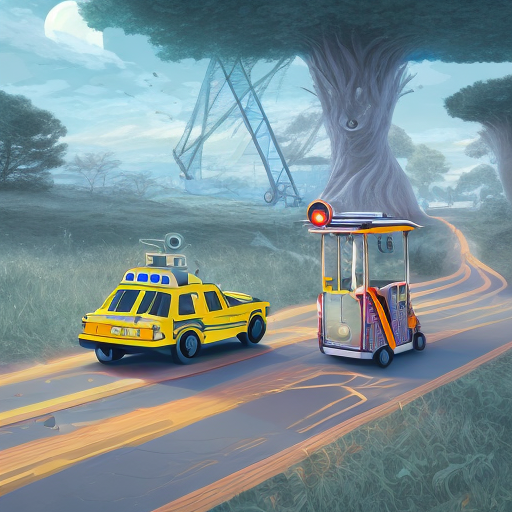
\includegraphics{trolley}
        \caption{"mdjrny-v4 A humorous, cartoonish illustration of an autonomous vehicle facing the classic trolley problem 8k" made with Stable Diffusion 2.1}
        \labfig{trolley}
\end{marginfigure}
\begin{pdf}

From a moral standpoint, the delegation of life-or-death decisions to machines raises profound questions about the nature of human agency and the limits of technological progress. As we continue to develop and deploy autonomous vehicles, it is crucial to engage in a broader societal conversation about the values and principles that should guide these advancements, ensuring that they serve the greater good while respecting individual rights and dignity.

The development of autonomous vehicles presents not only technological challenges but also complex ethical, legal, and moral dilemmas. By confronting these issues head-on, we can work towards a future where self-driving cars operate in harmony with human society, guided by shared values and a collective vision of progress.

\section{Driving Infrastructure}

As we delve deeper into the world of autonomous vehicles, it is essential to consider the broader infrastructure that supports these technologies. In this section, we will explore the challenges and opportunities related to maps, roads, sensors, software, and communications, shedding light on the complexities involved in creating a seamless, harmonious driving experience.

Maps play a crucial role in enabling autonomous vehicles to navigate their surroundings. However, one of the most significant challenges in map creation and maintenance is the concept drift – the ever-changing nature of our environments. Roads are altered, new construction projects arise, and traffic patterns shift. These changes can render maps outdated or inaccurate, as evidenced by the pileup crash cited in reference \sidecite{pileupcrash}, where a self-driving car's reliance on outdated map data contributed to the accident.

Roads and urban design are equally important when considering the infrastructure necessary for self-driving cars. Retrofitting cities to accommodate autonomous vehicles may involve the creation of dedicated lanes, the installation of new traffic signals, and the adaptation of pedestrian spaces to ensure the safe coexistence of humans and machines. These changes will require collaboration between urban planners, transportation experts, and policymakers to ensure that cities evolve in a manner that supports the widespread adoption of self-driving cars.

Sensors are the eyes and ears of autonomous vehicles, allowing them to perceive and interpret their surroundings. However, these sensors are not infallible – they can be impaired by dirt, debris, and other environmental factors. A dirty sensor can compromise a self-driving car's ability to function safely, emphasizing the need for regular maintenance and cleaning to ensure optimal performance.

Software plays a central role in the operation of autonomous vehicles, and while you might think that this software is all proprietary, there are many completely open source platforms like OpenPilot \cite{openpilot} leading the way in developing advanced driver assistance systems. However, questions surrounding the inspection, regulation, and potential bankruptcy of software providers must be addressed. Additionally, the risk of software failures, as demonstrated in the over-the-air (OTA) crash cited in reference \cite{otacrash}, highlights the need for robust safety mechanisms and regulatory oversight.

\begin{pdf}
\begin{marginfigure}[-5.5cm]
        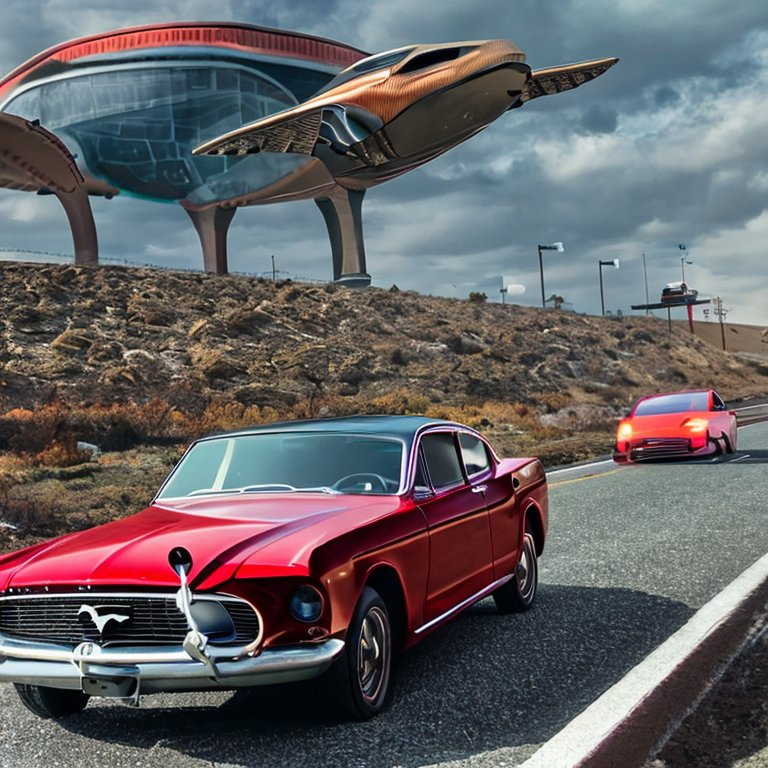
\includegraphics{mustang}
        \caption{"A steampunk scifi highway with a Tesla Model X driving next to a 1961 Ford Mustang" made with Stable Diffusion 2.1}
        \labfig{mustang}
\end{marginfigure}
\end{pdf}

Finally, communication is a vital aspect of autonomous driving infrastructure. Autonomous vehicles must be capable of communicating not only with other cars but also with people, animals, and various elements of the environment. The emergence of new technologies and trends, such as vehicle-to-vehicle (V2V) and vehicle-to-infrastructure (V2I) communication, has the potential to revolutionize the way self-driving cars interact with their surroundings. However, these advances also bring new challenges in terms of privacy, security, and standardization.

The development and adoption of autonomous vehicles are not solely dependent on the cars themselves but also on the supporting infrastructure. By addressing the challenges and seizing the opportunities presented by maps, roads, sensors, software, and communications, we can work towards a future where self-driving cars and human-driven vehicles coexist harmoniously within a dynamic, evolving transportation ecosystem.

\section{See You In Court!}

As autonomous vehicles become more prevalent, it is inevitable that their integration into society will bring legal challenges and disputes. In this section, we will examine the complexities of multicollinearity and mathematical chaos, explainability and accountability in court, and the role of trustworthy machine learning and inherently interpretable models in addressing these challenges.

Multicollinearity and mathematical chaos introduce an element of uncertainty in the performance of autonomous vehicles. As multiple, highly correlated variables affect the behavior of self-driving cars, determining the cause of a specific event can be difficult. This problem is exacerbated by the chaotic nature of the systems involved, where small changes in initial conditions can lead to vastly different outcomes. These factors can make it challenging to attribute responsibility in the event of an accident, particularly when attempting to disentangle the contributions of various components, such as hardware, software, and environmental factors.

\begin{pdf}
\begin{marginfigure}[-5.5cm]
        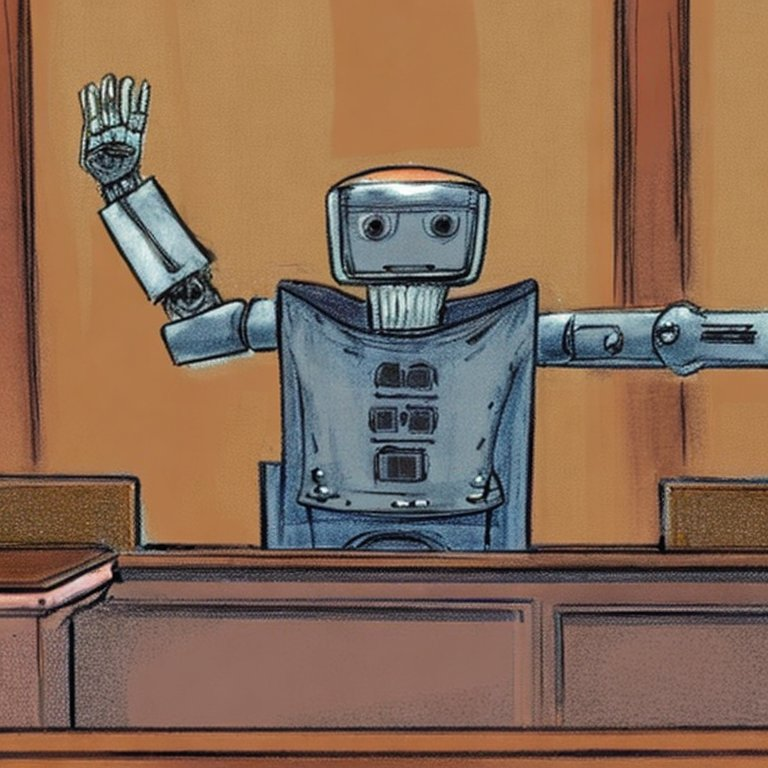
\includegraphics{robotcourt}
        \caption{"A courtroom sketch of a robot shrugging at the witness stand" made with Stable Diffusion 2.1}
        \labfig{robotcourt}
\end{marginfigure}
\end{pdf}

Explainability and accountability are critical concerns when presenting autonomous vehicle-related cases in court. If the decision-making processes of self-driving cars are inscrutable or difficult to understand, it becomes challenging to determine who or what is at fault in a given situation. This lack of transparency can impede the legal process and erode public trust in autonomous vehicle technology.

One potential solution to these challenges is the development of trustworthy machine learning, as described in Trustworthy ML\sidecite{trustworthyml}. By teaching developers to build models that are reliable, interpretable, and robust, we can create autonomous vehicles that are more easily understood and evaluated in legal proceedings. This approach prioritizes transparency and accountability, ensuring that the underlying algorithms driving these vehicles can be scrutinized and their decisions explained. 

In order to achieve explainability in artificial intelligence, it may be necessary to reconsider the recent advancements in deep neural networks. While these networks have demonstrated impressive performance, their opacity can make it difficult to understand how decisions are being made. This is where less advanced technology may have an advantage, as it allows for more transparency in the decision-making process. However, even with less advanced models such as decision trees, there is still the potential for complexity to create challenges in explainability. While theoretically fully explainable, decision trees can become cumbersome when they contain millions of lines of rules or code. As a result, they can be just as difficult to explain in a court of law as more advanced neural networks.

Inherently interpretable models further reinforce the case for transparency and accountability in autonomous vehicles. By developing machine learning models that are not only accurate but also readily interpretable, we can facilitate a more straightforward assessment of responsibility in the event of an accident. This clarity can help build public trust in the technology while also streamlining the legal process when disputes arise.

\section{Alternative Approaches}

As we explore the future of autonomous vehicles, it is crucial to consider alternative ways of thinking about self-driving cars and their potential roles in our transportation ecosystem. In this section, we will discuss various concepts that challenge conventional notions of autonomy and offer novel solutions that could complement or transform our understanding of mobility.

One alternative approach involves reimagining self-driving cars as a form of "train" that operates in dedicated lanes. By constructing special lanes for autonomous vehicles, we can essentially put these cars "on rails," enabling them to function more like a train. This approach would not only enhance the safety and efficiency of autonomous vehicles but also provide a glimpse into the potential infrastructural and regulatory frameworks necessary for their success.

In the realm of logistics and warehousing, the lack of self-driving forklifts offers an interesting lesson. Instead of focusing on automating forklifts, warehouses have implemented moving shelves, essentially flipping the problem on its head to achieve a more efficient solution. This example highlights the importance of rethinking traditional approaches to autonomy and searching for innovative ways to streamline various aspects of our economy.

\begin{pdf}
\begin{marginfigure}[-5.5cm]
        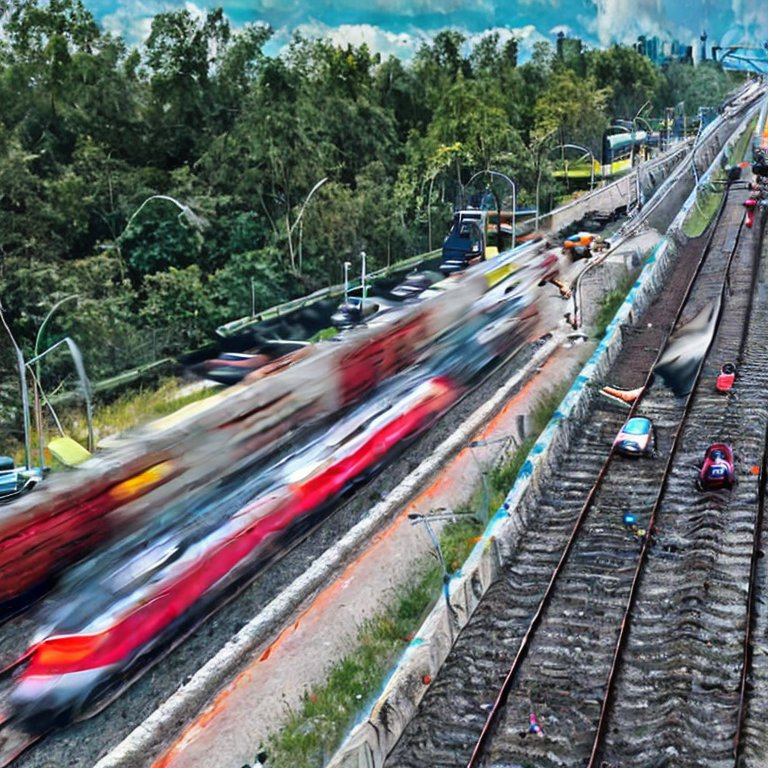
\includegraphics{trains}
        \caption{"trains going down the highway next to cars, bicycles and scooters" made with Stable Diffusion 2.1}
        \labfig{trains}
\end{marginfigure}
\end{pdf}

Building on these ideas, we can explore other unconventional approaches that challenge the status quo of autonomous vehicles. One possibility is the development of platooning systems, in which multiple vehicles travel in close proximity, communicating with one another to maintain safety and optimize traffic flow. This approach could harness the advantages of vehicle-to-vehicle communication while reducing the need for extensive infrastructure modifications.

Another alternative is the concept of supervised autonomy, not from the driver at a moment's notice like we have today, but from a control tower similar to those used at airports. This has large privacy implications but combines the benefits of autonomous technology with human oversight. This approach allows for human intervention in complex or high-risk situations, mitigating concerns about delegating life-or-death decisions to machines while still reaping the rewards of autonomous driving.

In all these alternative approaches, the key is to think creatively about how we can integrate self-driving cars into our transportation systems. By challenging conventional wisdom and exploring innovative solutions, we can create a more efficient, sustainable, and harmonious future for transportation, one that redefines the role of autonomous vehicles within an ever-evolving paradigm.

\section{Key Takeaways}

\begin{itemize}
\item \textbf{Redefine autonomy with alternative approaches:} Consider dedicated lanes, supervised autonomy, and other unconventional methods to enhance safety and efficiency while reimagining the role of self-driving cars in our transportation systems.
\item \textbf{Adapt to ever-changing driving infrastructure:} Address challenges in maps, roads, sensors, software, and communications to create a seamless, harmonious driving experience, while ensuring regular maintenance and updates. Embrace open-source software and standardized solutions to foster collaboration and innovation.
\item \textbf{Prioritize explainability and accountability:} Develop trustworthy machine learning and inherently interpretable models to enhance transparency, facilitate legal proceedings, and build public trust in autonomous vehicle technology.
\item \textbf{Leverage communication and collaboration:} Promote vehicle-to-vehicle communication, coordination with external systems, and remote control for improved safety, efficiency, and adaptability in a dynamic transportation environment. Encourage the adoption of industry standards to facilitate interoperability and streamline implementation.
\item \textbf{Balance innovation with regulation:} Establish robust regulatory frameworks that protect privacy, maintain accountability, and ensure safety while fostering technological advancements, and integrating autonomous vehicles into our evolving transportation landscape.
\end{itemize}
